\documentclass{article}
\usepackage{graphicx, float}
\usepackage{enumitem}
\usepackage[hidelinks]{hyperref}

\graphicspath{{images/}}
\author{Cristian Di Cintio - S1110150 \and Federico Di Giovannangelo - S0000000}
\date{}

\title{READING STATS\par \large RELAZIONE DI PROGRAMMAZIONE MOBILE}


\begin{document}

\maketitle
\tableofcontents
\newpage

\section{Introduzione}

L'applicazione sviluppata ha come obiettivo la memorizzazione delle statistiche di libri in lettura dell'utente. Tali statistiche riguardano la percentuale di completamento del libro e il tempo impiegato, memorizzato per ciascuno libro.

L'utente per usufruire delle funzionalità dell'app deve registrarsi con nome, cognome, email, username e password. Per lo username e l'email vengono effettuati dei controlli per verificare l'univocità e non permettere la registrazione di utenti con medesimo username o email.

In seguito l'utente può effettuare l'accesso con la propria email e password.

L'utente può ricercare i libri in un catalogo tramite la digitazione del titolo in una barra di ricerca o scansionando, con un pulsante apposito, il codice a barre di un libro fisico. In seguito può decidere di aggiungerlo in tre liste distinte, "da leggere", "in lettura" e "letti", 
per avere un resoconto delle pagine lette e del tempo impiegato nella lettura dei libri salvati. Il catalogo permette anche il filtraggio di libri tramite la selezione di categorie predefinite.

Al momento della lettura l'utente può avviare un timer per un libro in lettura, presente nell'omonima lista, e disattivarlo al termine della sessione.

L'utente può visualizzare e modificare i propri dati personali e interagire con altri utenti, visualizzando principalmente quali libri hanno salvato e quali stanno leggendo, ognuno con le loro rispettive metriche.

L'intera applicazione è stata sviluppata inizialmente in Kotlin per ambiente Android e in seguito in Flutter per un funzionamento multipiattaforma, in modo tale da permettere una maggiore compatibilità e una migliore interazione tra utenti con diversi dispositivi mobile.

Lo sviluppo in Kotlin è stato applicato con Jetpack Compose, per permettere uno sviluppo moderno e in linea con le attuali applicazioni sul mercato, con una struttura architetturale basata sul Model-View-ViewModel (MVVM) garantendo una composizione comprensibile per lo sviluppo dell'app.
Le informazioni principali dei libri vengono visualizzate tramite l'utilizzo di API fornite da Google Books.

\section{Progettazione e sviluppo Android}

\subsection{Requisiti e casi d'uso}
Si riportano di seguito i requisiti \textit{funzionali} e \textit{non funzionali}
\subsubsection{Requisiti funzionali}

\begin{figure}[H]
  \centering
  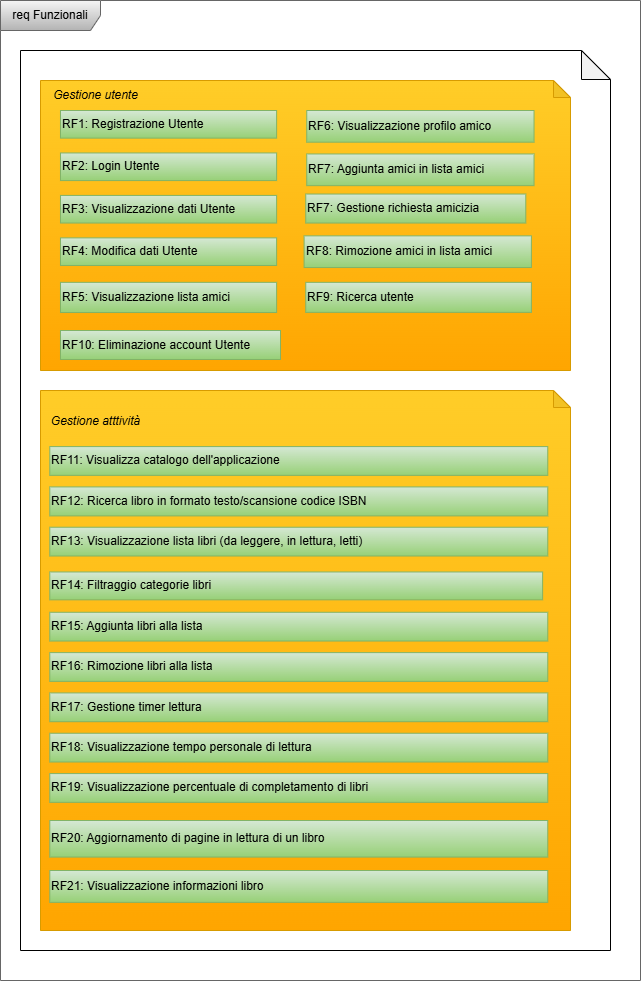
\includegraphics[width=.9\linewidth]{req_funzionali.png}
  \caption{Requisiti funzionali}
  \label{fig:sitemap}
\end{figure}

\begin{itemize}
    \item \textit{Gestione utente}
    \begin{itemize}
        \item \textit{RF1: Registrazione utente} - L'applicazione permette di registarsi con le proprie informazioni personali
        \item \textit{RF2: Login utente} - L'applicazione permette di autenticare l'utente registrato con le proprie informazioni personali
        \item \textit{RF3: Visualizzazione dati utente} - L'applicazione permette di visualizzare i propri dati personali
        \item \textit{RF4: Modifica dati utente} - L'applicazione permette di modificare i propri dati personali
        \item \textit{RF5: Visualizzazione lista amici} - L'applicazione permette di visualizzare la lista degli amici che hanno accettato la sua richiesta d'amicizia
        \item \textit{RF6: Visualizzazione profilo amico} - L'applicazione permette di visualizzare il profilo di un suo amico nella lista
        \item \textit{RF7: Aggiunta amici in lista amici} - L'applicazione permette di aggiungere un amico nella sua lista inviando una richiesta
        \item \textit{RF8: Gestione richiesta di amicizia} - L'utente può decidere se accettare o rifiutare una richesta di amicizia
        \item \textit{RF9: Rimozione amici da lista amici} - L'applicazione permette di rimuovere un amico dalla lista amici
        \item \textit{RF10: Ricerca utente} - L'applicazione permette di ricercare un utente digitando il suo username o nome completo
        \item \textit{RF11: Eliminazione account utente} - L'applicazione permette all'utente di cancellare il proprio profilo
    \end{itemize}
    \item \textit{Gestione attività}
    \begin{itemize}
        \item \textit{RF12: Visualizza catalogo dell'applicazione} - L'applicazione permette di visualizzare il catalogo dei libri distinti in categorie
        \item \textit{RF13: Ricerca libro in formato testo o tramite scansione codice a barre} - L'applicazione permette la ricerca del libro digitando testualmente il titolo in una casella di ricerca apposita oppure scansionando il codice a barre di un libro fisico
        \item \textit{RF14: Visualizzazione lista libri (da leggere, in lettura, letti)} - L'applicazione permette di visualizzare il contenuto delle liste principali formate dai libri salvati dall'utente
        \item \textit{RF15: Filtraggio categorie libri} - L'applicazione permette all'utente di filtrare le categorie dei libri da visualizzare nel catalogo 
        \item \textit{RF16: Aggiunta libri alla lista} - L'applicazione permette all'utente di aggiungere i libri in una delle apposite liste fornite dall'app
        \item \textit{RF17: Rimozione libri dalla lista} - L'applicazione permette la rimozione di libri dalle liste
        \item \textit{RF18: Gestione timer lettura} - L'applicazione permette di tenere sotto controllo il tempo di lettura di un libro con l'utilizzo di un timer dedicato attivabile e disattivabile dall'utente
        \item \textit{RF19: Visualizzazione tempo personale di lettura} - L'applicazione permette all'utente di visualizzare per ogni singolo libro il tempo di lettura impiegato con l'utilizzo del timer
        \item \textit{RF20: Visualizzazione percentuale completamento di libri} - L'applicazione permette di visualizzare la percentuale di completamento di ogni singolo libro, calcolata tramite il numero di pagine lette dall'utente rispetto al numero di pagine totali di un determinato libro
        \item \textit{RF21: Aggiornamento percentuale di pagine in lettura di un libro} - L'applicazione permette di aggiornare il numero di pagine lette di un libro per calcolare la percentuale di completamento
        \item \textit{RF22: Visualizzazione informazioni libro} - L'applicazione permette la visualizzazione delle info di un determinato libro 
    \end{itemize}
\end{itemize}

\subsubsection{Requisiti non funzionali}

\begin{figure}[H]
  \centering
  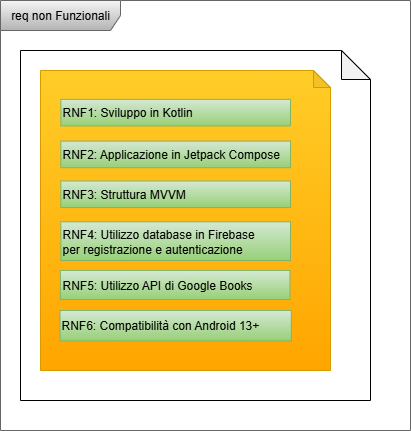
\includegraphics[width=.6\linewidth]{req_non_funzionali.png}
  \caption{Requisiti non funzionali}
  \label{fig:sitemap}
\end{figure}

\begin{itemize}[label=\textendash]
    \item \textit{RNF1: Sviluppo in Kotlin} - L'applicazione è stata sviluppata principalmente con il linguaggio di programmazione Kotlin
    \item \textit{RNF2: Applicazione in Jetpack Compose} - L'applicazione è stata realizzata con Jetpack Compose per realizzare le interfacce grafiche
    \item \textit{RNF3: Struttura MVVM} - L'applicazione ha una struttura architetturale basata su Model-View-ViewModel per agevolare la programmazione con sezioni dedicate
    \item \textit{RNF4: Firebase Firestore per memorizzazione e accesso/autenticazione utente} - L'applicazione fa utilizzo per la memorizzazione di dati e la gestione della registrazione e l'accesso dell'utente di un database tramite la piattaforma Google Firebase
    \item \textit{RNF5: API di Google Books} - L'applicazione si sincronizza e fa utilizzo delle API Key di Google Books per mostrare i libri nel catalogo e nella ricerca
    \item \textit{RNF6: compatibilità con Android 13+} - L'applicazione ha una compatibilità con il livello di API 33, permettendone l'utilizzo su android 13 e oltre
\end{itemize}

\subsubsection{Casi d'uso}
Si riportano gli attori e i tre casi d'uso principali che descrivono le azioni principali che si possono svolgere nell'applicazione a partire dai requisiti elencati in precedenza.

\begin{figure}[H]
  \centering
  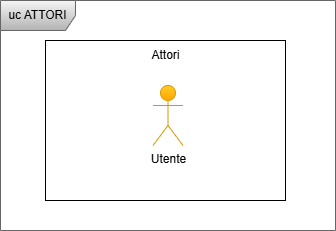
\includegraphics[width=.6\linewidth]{cu_attori.png}
  \caption{Attori principali}
  \label{fig:sitemap}
\end{figure}

\begin{figure}[H]
  \centering
  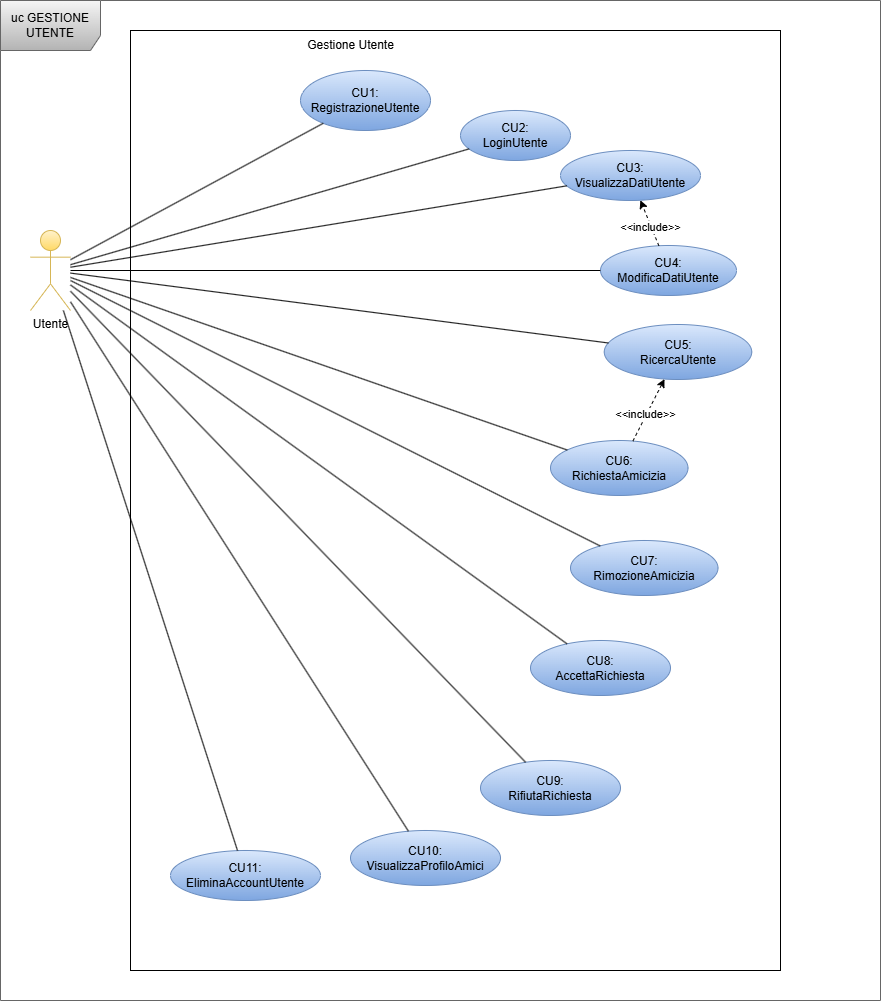
\includegraphics[width=.8\linewidth]{cu_utente.png}
  \caption{Gestione utente}
  \label{fig:sitemap}
\end{figure}

\begin{itemize}[label=\textendash]
    \item \textit{CU1: RegistrazioneUtente} - L'utente, per usufruire dei servizi offerti dall'applicazione, ha bissogno di registarsi con le proprie informazioni personali
    \item \textit{CU2: LoginUtente} - L'utente può accedere ai servizi forniti inserendo le proprie credenziali (email e password) precedentemente utilizzate per registrarsi
    \item \textit{CU3: VisualizzaDatiUtente} - L'utente può visualizzare le proprie informazioni personali in una sezione dedicata
    \item \textit{CU4: ModificaDatiUtente} - L'utente può modificare i propri dati personali
    \item \textit{CU5: RicercaUtente} - L'utente può ricercare un utente digitando il suo nome utente (usernam) o nome completo (nome e/o cognome)
    \item \textit{CU6: RichiestaAmicizia} - L'utente può aggiungere amici nella propria lista inviando richieste ad altri utenti
    \item \textit{CU7: RimozioneAmicizia} - L'utente può rimuovere gli amici dalla propria lista
    \item \textit{CU8: AccettaRichiesta} - L'utente può accettare la richiesta di amicizia da un altro utente che l'ha inviata
    \item \textit{CU9: RifiutaRichiesta} - L'utente può rifiutare la richiesta di amicizia da un altro utente che l'ha inviata
    \item \textit{CU10: VisualizzaProfiloAmici} - L'utente può visualizzare il profilo dei propri amici con le loro statistiche di lettura
    \item \textit{CU11: EliminaAccountUtente} - L'utente può eliminare il proprio account utente
\end{itemize}

\begin{figure}[H]
  \centering
  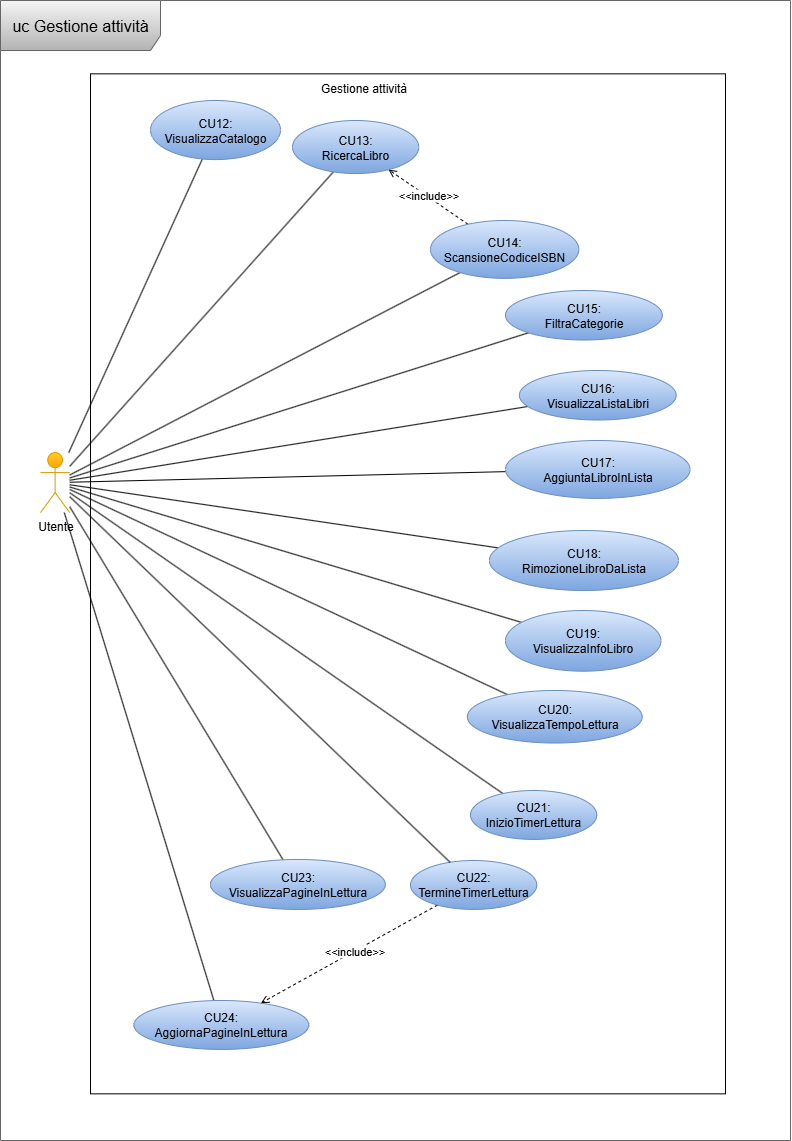
\includegraphics[width=0.72\linewidth]{cu_attivita.png}
  \caption{Gestione attività}
  \label{fig:sitemap}
\end{figure}

\begin{itemize}[label=\textendash]
    \item \textit{CU12: VisualizzaCatalogo} - L'utente può visualizzare il catalogo di libri separato in categorie
    \item \textit{CU13: RicercaLibro} - L'utente può ricercare il libro digitando il titolo nella barra di ricerca presente nel catalogo
    \item \textit{CU14: ScansioneCodiceISBN} - L'utente può effettuare la scansione del codice ISBN di un libro fisico tramite la fotocamera del telefono
    \item \textit{CU15: FiltroCategorie} - L'utente può filtrare le categorie del catalogo selezionandole da un lista con checkbox
    \item \textit{CU16: VisualizzaListaLibri} - L'utente può visualizzare una delle tre liste principali (da leggere, in lettura, letti) per memorizzare i libri salvati
    \item \textit{CU17: AggiuntaLibroInLista} - L'utente può aggiungere un libro selezionato in una delle tre liste principali (da leggere, in lettura, letti)
    \item \textit{CU18: RimozioneLibroDaLista} - L'utente può rimuovere un libro presente in una delle tre liste principali (da leggere, in lettura, letti)
    \item \textit{CU19: VisualizzaInfoLibro} - L'utente può visualizzare le informazioni principali che rappresentano il libro selezionandolo dal catalogo o dalle liste
    \item \textit{CU20: VisualizzaTempoLettura} - L'utente può visualizzare il tempo di lettura di un proprio libro
    \item \textit{CU21: InizioTimerLettura} - L'utente può iniziare la sessione di lettura di un libro tramite l'inizio di un timer dedicato
    \item \textit{CU22: TermineTimerLettura} - L'utente può terminare la sessione di lettura di un libro permettendo di fermare il timer
    \item \textit{CU23: VisualizzaPagineInLettura} - L'utente può visualizzare le pagine in lettura di un libro salvato nell'omonima lista
    \item \textit{CU24: AggiornaPagineInLettura} - L'utente può aggiornare le pagine 
\end{itemize}

\subsection{Architettura applicazione}

\subsubsection{MVVM}

Per la struttura dell'applicazione è stato scelto il pattern architetturale Model-View-ViewModel (MVVM) per ottenere
una separazione netta delle responsabilità tale da rendere il codice scalabile e facilmente aggiornabile.
Le sue principali componenti sono:
\begin{itemize}
  \item \textbf{Model:} Gestisce i dati dell'applicazione e della loro persistenza, principalmente in remoto con Firebase nel caso specifico di questa applicazione, 
  permettendo operazioni di accesso, modifica e salvataggio dei dati per gli \textit{utenti} che si registrano e dei \textit{libri} che salvano in determinate liste. 
  \item \textbf{View:} Rappresenta le interfacce dell'applicazione per permettere all'utente di interagire con la logica dell'applicazione. 
  Vengono definite tramite funzioni con la notazione iniziale \textit{@Composable} e possono essere richiamate nel file contenente il MainActivity o in altre funzioni con la stessa notazione.
  \item \textbf{ViewModel:} Funge da intermediario tra View e Model e permette il cambiamento dello stato della UI con le interazioni dell'utente tramite \textit{LiveData}
\end{itemize}

\subsubsection{Diagramma delle componenti}

Il seguente diagramma di componenti rappresenta le principali istanze e le loro interazioni, in particolare tra l'utente e un singolo libro scelto, la lista dei libri e la richiesta di amicizia verso un altro utente.
Per il libro l'utente può decidere se inserirlo in una lista o rimuoverlo, mentre per la richiesta l'utente può inviarne una e visualizzarne una ricevuta, per poi decidere se accettarla o rifiutarla.

\begin{figure}[H]
  \centering
  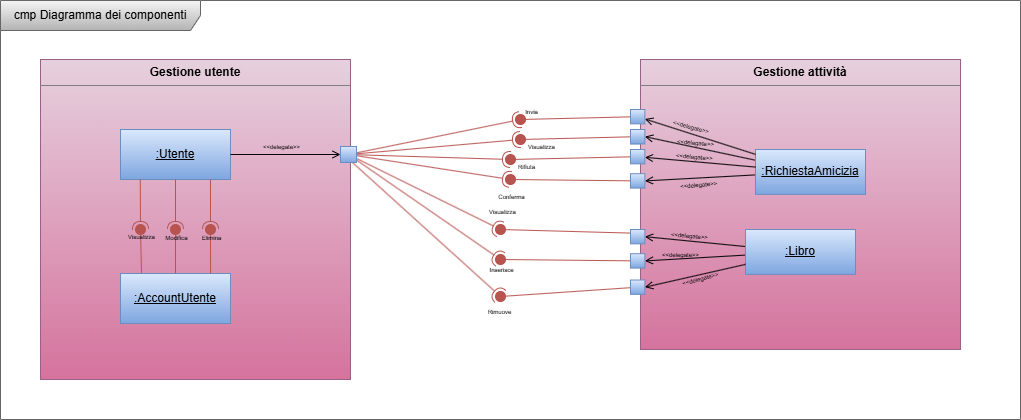
\includegraphics[width=1\linewidth]{diagramma_componenti.png}
  \caption{Diagramma delle componenti}
  \label{fig:sitemap}
\end{figure}

\subsection{Gestione Database - Firebase}
In presenza di un sistema di autenticazione e registrazione a un servizio online, con la possibilità per l'utente di interagire con altri utenti, e permettere il salvataggio personale di libri nel proprio profilo,
l'infrastruttura migliore per manipolare questi dati risulta essere il database gestionale Firestore di Google Firebase.

Firestore è un DB NoSQL strutturato a documenti, il quale permette il salvataggio di dati in documenti raggrupati in collezioni e può contenere sottocollezioni e campi annidati. Tali documenti e collezioni vengono generati con la scrittura di dati tramite codice.

Il suo utilizzo si concentra su due componenti della sezione \textit{Creazione}:
\begin{itemize}
  \item \textit{Authentication:} permette di gestire il metodo di accesso degli utenti tramite diversi servizi. Nel caso di questo progetto abbiamo implementato esclusivamente l'autenticazione semplice tramite email e password.
    \begin{figure}[H]
    \centering
    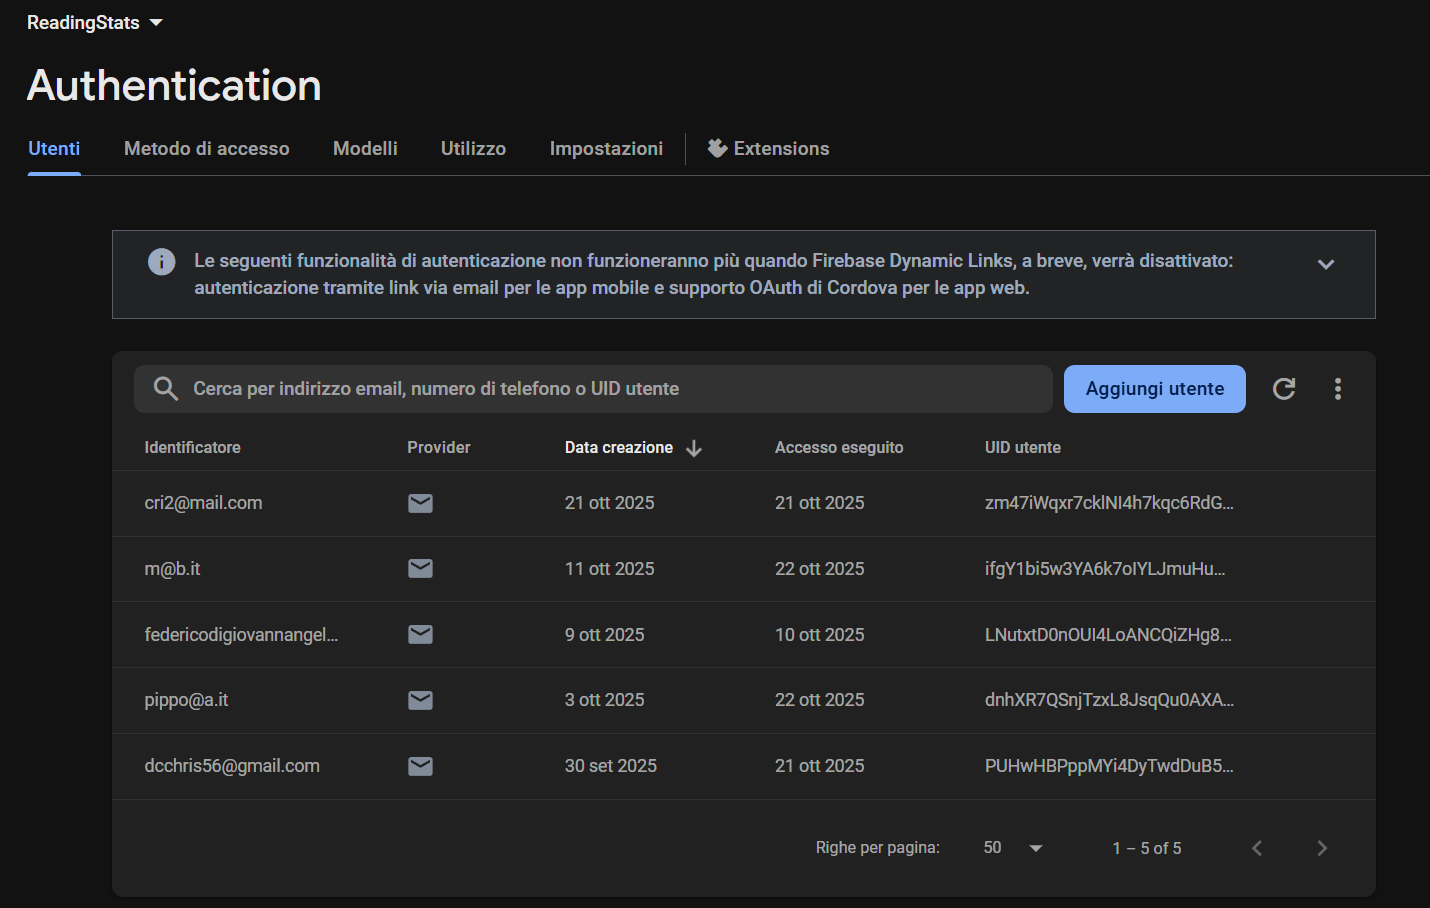
\includegraphics[width=1\linewidth]{authentication.png}
    \caption{Diagramma delle componenti}
    \label{fig:sitemap}
  \end{figure}
  \item \textit{Firestore Database:} permette la memorizzazione tramite documenti e collezioni descritti in precedenza dei dati dell'utente, delle richieste di amicizia inviate tra utenti e dei libri salvati con ognuno la relativa sessione. 
  Sono state implementate delle regole specifiche per permettere un corretto e coerente accesso ai dati e la loro relativa modifica. Di seguito i documenti e le collezioni generate:
  
  \textit{INSERIRE SCREEN PER OGNI SEZIONE}

  \begin{itemize}
    \item \textbf{Salvataggio utenti:} Utenti registrati e salvati nel servizio tramite il form di registrazione, memorizzando nome, cognome, username e mail;
    \item \textbf{Salvataggio usernames:} Username salvati al momento della registrazione per permettere un controllo di univocità;
    \item \textbf{Salvataggio di amici tramite richieste:} Lista di utenti che si aggiorna per ogni singolo utente quando accetta una richiesta di amicizia da un altro utente;
    \item \textbf{Salvataggio di libri dal catalogo:} Raccolta di libri salvati per ogni utente, ognuno con le sue informazioni e lo stato per visualizzarlo in una determinata lista tra quelle fornite;
    \item \textbf{Salvataggio sessione di lettura:} Per ogni libro nello stato "In lettura", viene memorizzata una sessione di lettura contenente il tempo memorizzato in secondi e convertito a schermo in ore:minuti:secondi;
    \item \textbf{Regole di accesso ai documenti definiti:} Le seguenti regole scritte nell'omonima sotto-sezione permettono la definizione di un accesso; 
  \end{itemize} 
\end{itemize}



\subsection{API utilizzate - Google Books}
Le API di Google Books sono state utilizzata per ottenere le informazioni principali dei libri, in modo da permettere
all'utente la loro visualizzazione e il conseguente salvataggio. L'API viene fornita tramite un link 
per le ricerche e una chiave generata da Google Cloud per permetterne l'abilitazione e la limitazione del tipo di dispositivo che la utilizzerà.

\textit{Link:  https://www.googleapis.com/books/v1/volumes?q=search-terms}.

\textit{"q"} è il parametro da inserire per effettuare la ricerca tramite titolo o autore. Sono presenti altri parametri, i cui principali per l'applicazione sono stati:
\begin{itemize}
  \item \textit{maxResults}, per mostrare la quantità di libri da visualizzare, utilizzato in particolare nel catalogo e nella ricerca.
  \item \textit{orderBy}, il quale può essere relevance o newest per mostrare libri di maggiore rilievo tramite parametriche di Google o nuove uscite.
  \item \textit{langRestrict}, ossia la restrizione dei libri da visualizzare e ricercare con la una lingua specifica.
\end{itemize}


\subsection{Sviluppo}
Come anticipato in precedenza, l'applicazione è interamente sviluppata in \textbf{Jetpack Compose}, un toolkit dichiarativo di Android che permette, al variare del proprio stato, di ridisegnare le parti necessarie al cambiamento di tale stato.

Permette un approccio dichiarativo tramite la definizione di funzioni con notazione \textit{@Composable}, le quali permettono di definire parti di interfaccia utente esclusivamente con codice Kotlin. 
In queste funzioni si controlla lo stato per permettere l'aggiornamento di determinate parti coinvolte.

Sono disponibili una serie di layout predefiniti (Column, Row, Box) per strutturare al meglio una componente dell'interfaccia e le funzioni accettano un parametro Modifier che permette di modificarne l'aspetto estetico.

Per la costruzione di un'interfaccia tradizionale è stato utilizzata la funzione \textit{Scaffold} con parametri per definire componenti predefinite come TopAppBar, BottomAppBar, FloatingActionButton e altri ancora.

Si possono distinguere due tipi di funzioni Composable:
\begin{itemize}
  \item \textbf{Stateful}, fa utilizzo della keyword \textit{remember} che permette di memorizzare dati tra diverse recomposition
  \item \textbf{Steless}, ossia un Composable orivo di stato
\end{itemize}

Le liste scorrevoli che visualizzano molti elementi vengono gestite da componenti \textit{Lazy}, che forniscono un blocco per descrivere i singoli \textit{item} da visualizzare.  
Ne esistono diverse versioni:
\begin{itemize}
  \item \textbf{LazyRow} per lo scorrimento orizzontale,
  \item \textbf{LazyColumn} per lo scorrimento verticale,
  \item \textbf{LazyVerticalGrid e LazyHorizontalGrid} per lo scorrimento di una griglia rispettivamente verticale e orizzontale
\end{itemize}

La navigazione viene principalmente gestita tramite un file dedicato, denominato \textbf{AppNavHost.kt},
nel quale viene creato un \textit{NavController} e un \textit{NavHost},
il quale fa uso della funzione \textit{composable} che permette di definire le rotte di destinazione
all'interno dell'applicazione. Tali rotte vengono definite in formato di stringa in un altro file denominato \textbf{Routes.kt} 

Le funzioni con notazione \textit{@Composable} possono essere richiamate da un Activity o Fragment, da altre funzioni \textit{@Composable}, 
all'interno di una destinazione definita in Navigation-Compose e in liste Lazy.

\subsubsection{Struttura package}
Il progetto, strutturato con architettura MVVM, è stato suddiviso in macro-package al cui interno sono presenti file o altri package caratteristici.

La struttura delle macro-cartelle risulta la seguente:

\begin{itemize}
  \item \textbf{core:} contiene i package con i file di parti di interfaccia
  \textit{@Composable} riutilizzabili nel codice e i file utilizzati per la personalizzazione globale dell'app.
  \item \textbf{di:} moduli di \textit{Dependency Injection} (Hilt) che descrivono come creare e fornire le dipendenze dell’app. 
  Le classi ricevono gli oggetti necessari tramite iniezione, senza istanziarli al proprio interno. 
  Contiene i file usati a livello globale per integrare le Google Books API e configurare lo stack di rete.
  \item \textbf{features:} è presente il codice principale dell'applicazione scritto in diversi file distinti e gestito in package annidati per la loro funzionalità nell'applicazione.
  \item \textbf{navigation:} contiene i file di gestione della navigazione e di creazione delle route.
\end{itemize}

\subsubsection{File di configurazione}

Sono stati modificati i file di configurazione per l'importazione di diverse dipendenze nel progetto.
I principali file sono:

\begin{itemize}
  \item \textbf{AndroidManifest.xml:} Utilizzato per la dichiarazione di diversi componenti e permessi per l'app sviluppata su Android che riconosce in runtime.
  Il principale permesso applicato è stato INTERNET per permettere la richiesta via rete di libri tramite le API fornite.
  \item \textbf{build.gradle.kts (app):} Definisce la modalità di compilazione del modulo \textit{app} e quali librerie collegare per il loro utilizzo. A differenze di AndroidManifest, viene valutato a build-time.
  \item \textbf{build.gradle.kts (root):} Permette l'applicazione di configurazioni e impostazioni condivise a tutti i moduli.
\end{itemize}

\subsection{Spiegazione codice in dettaglio}
Di seguito, viene suddivisa in sezioni la spiegazione nel dettaglio dello scopo dei file con le proprie componenti utilizzate.

\subsubsection{core: Componenti Compose riutilizzabili}
In questo package troviamo componenti \textit{@Compose} riutilizzabili nel codice, elencati e descritti di seguito:

\begin{itemize}
  \item \textbf{AppScaffold.kt:} Struttura principale del componente Scaffold dell'applicazione, con parametri \textit{topBar} e \textit{bottomBar} assegnati in \textbf{AppNavHost.kt}. Permette la definizione della struttura principale dell'applicazione.
  \item \textbf{HeaderComponent.kt:} Struttura dell'intestazione dell'app, costruita con \textit{TopAppBar}, contenente il logo dell'applicazione e il titolo "Reading Stats".
  \item \textbf{NavBarComponent.kt:} Struttura della barra di navigazione per permettere di navigare tra le quattro sezioni principali dell'applicazione: \textbf{Scaffali, Catalogo, Home e Profilo}. Al richiamo con il parametro assegnato di tipo \textit{NavController}, viene assegnata poi al parametro bottomBar di AppScaffold. 
  \item \textbf{SerchBar.kt:} Barra di ricerca costruita e utilizzata nella schermata del \textbf{Catalogo} e nella sezione \textit{Amici} del \textbf{Profilo}, rispettivamente utilizzata per la ricerca di libri o per la ricerca di amici registrati all'applicazione.
  \item \textbf{VerticalScrollBar.kt:} Barra di scorrimento verticale richiamata nella finestra di dialogo per la selezione dei filtri del \textbf{Catalogo}.
\end{itemize}

\subsubsection{di: Dependency Injection}
Tale package racchiude i moduli \textbf{Hilt} che dichiarano come costruire le dipendenze dell'app a runtime, come \textit{Firebase, Retrofit e OkHttp}. Permette quindi una configurazione centralizzata e una migliore testabiità dell'intera app.

\begin{itemize}
  \item \textbf{AuthModule.kt:} permette la definizione e l'iniziezione nei ViewModel della catena \textbf{UseCase → Repository → DataSource → Firebase}.
  Fornisce servizi di base per l'autenticazione e l'estrazione di dati da database Firestore. Sono presenti degli use case per il login, la registrazione e il controllo dello username.
  Fa uso di due annotazioni:
  \begin{itemize}
    \item \textit{@Singleton:} Annotazione di scope per mantenere una sola istanza del binding per il tempo di vita del componente su cui è installato.
    \item \textit{@InstallIn:} Annotazione di installazione di modulo il quale comunica con Hilt a quale componente deve essere unito il modulo (con annotazione \textit{@Module}) che contiene le notazioni \textit{@Provides o @Bind}.
    Definisce quindi il raggio d'azione del modulo e la visibilità dei binding.
  \end{itemize}
  \item \textbf{NetworkModule.kt:} Permette la configurazione di rete dell'applicazione e la possibilità di richiedere le informazioni dei libri tramite l'url fornito dalle API di Google Books.
  \item \textbf{KeysModule.kt:} Definisce un qualifier \textit{@BooksApiKey} per evitare collisioni tra generiche String e la chiave fornita da Google Books quando viene iniettata.
\end{itemize}

\subsubsection{Package interni a features}
Di seguito vengono elencati e descritti lo scopo dei singoli package contenuti in \textbf{features}, 
utilizzati per distinguere le diverse sezioni dell'applicazione. Ognuno di loro contiene a sua volta dei package per l'applicazione della struttura con MVVM, quindi con schermate definite con funzioni \textit{@Composable} e model per rappresentare classi i cui oggetti saranno memorizzati nel database Firestore.
\begin{itemize}
  \item \textbf{auth:} contiene ulteriori package con file per la corretta gestione dell'accesso e della registrazione dell'utente tramite Firestore.
  \item \textbf{bookdetail:} contiene i file di schermata delle info del libro selezionato dal catalogo o dalla lista dei libri salvati nel proprio scaffale, con un view model dedicato alla gestione del salvataggio nelle liste e all'aggiornamento delle pagine lette.
  \item \textbf{catalog:} contiene ulteriori package con file per la visualizzazione e gestione del catalogo di libri, richiamando grazie al proprio view-model la possibilità di effettuare query per l'estrazione di libri.
  \item \textbf{home:} contiene ulteriori package con file per la sezione home, la quale permette di visualizzare e interagire con i libri salvati nella lista "In lettura" in modo da permettere l'avvio di un timer dedicato per ciascuno di loro.
  \item \textbf{profile:} contiene ulteriori package con file per la gestione del profilo utente, nel quale è possibile visualizzare le proprie informazioni e visualizzare le informazioni relative agli utenti amici.
  \item \textbf{shelves:} contiene ulteriori package con file per gestione della sezione "scaffali", contenente le liste di libri salvati dall'utente distinte in tre categorie: \textit{da leggere, in lettura e letti}
\end{itemize} 

\subsubsection{File di sorgente per gestione autenticazione}
I seguenti file sono utilizzati per la gestione dell'accesso e della registrazione dell'utente nel database Firestore.
\begin{itemize}
  \item \textbf{FirebaseAuthDataSource.kt:} Sorgente dati che incapsula \textit{FirebaseAuth} per operazioni di autenticazione. 
  Espone funzioni sospese \textit{createUser(email, password)} e \textit{signIn(email, password)} (ritornano \textit{AuthResult} usando \textit{await()}), oltre a metodi sincroni \textit{signOut()} e \textit{currentUid()} per terminare la sessione e ottenere l’UID corrente.

  \item \textbf{FirestoreUserDataSource.kt:} Sorgente dati che incapsula \textit{FirebaseFirestore} per la gestione dei profili utente, usando le collezioni \textit{users} e \textit{usernames}. 
  Fornisce \textit{isUsernameTaken(username)} e \textit{userExists(uid)}; \textit{createUserAtomically(uid, profile)} esegue una transazione che verifica collisioni sullo username e registra in modo coerente sia il documento utente sia il mapping username\,$\rightarrow$\,uid (merge con \textit{SetOptions}). \textit{getUserProfile(uid)} legge e mappa il documento in \textit{UserModelDto}. \textit{updateUserProfile(uid, username, name, surname, email)} aggiorna i campi (incluso \textit{updatedAt}) e, in transazione, se lo username cambia rimuove il vecchio mapping in \textit{usernames}, verifica che il nuovo non sia occupato e crea il nuovo mapping prima di aggiornare il documento in \textit{users}; eventuali eccezioni sono rilanciate per la gestione a livello ViewModel.

\end{itemize}

\subsubsection{Model: file principali}
I Model dell'applicazione vengono qui descritti distinguendo i package interni di \textbf{features}, i quali sono:
\begin{itemize}
  \item \textbf{auth:}
  \begin{itemize}
    \item \textbf{data.model.UserModelDto.kt:} descrive le componenti principali dell'utente che si registra e fa uso del servizio.
    Viene denotato con \textit{DTO} per indicare Data Transfer Object, ossia una classe contenitore utilizzata per trasportare informazioni tra diversi processi.
    In questo caso viene utilizzata per la gestione delle informazioni da salvare per gli utenti nel database Firestore.
    \item \textbf{domain.model:}
    \begin{itemize}
      \item \textbf{LoginFormState.kt:} File di rappresentazione dello stato per il login dell'utente che accede, contenente quindi le informazioni essenziali per il suo accesso e la conseguente verifica.
      \item \textbf{RegisterFormState.kt:} Rispetto a LoginState, questo file contiene più informazioni necessarie per la memorizzazione per la memorizzazione dell'utente nel servizio.
    \end{itemize}
  \end{itemize}
  \item \textbf{catalog:}
  \begin{itemize}
    \item \textbf{data.dto.GoogleBooksDto.kt:} contiene determinati DTO per Google Books, utilizzati per la loro ricerca e l'estrazione delle informazioni principali.
    \item \textbf{domain.model.Book.kt:} Model principale del libro, utilizzato per definire e raccogliere le informazioni estratte e richiamarle da un oggetto istanziato.
  \end{itemize}
  \item \textbf{home:}
  \begin{itemize}
    \item \textbf{domain.model.UiHomeBook.kt:} Model del libro per la sezione home, contenente le informazioni principali del libro, il numero di pagine lette registrate dall'utente (attributo \textit{pageInReading}) e il totale dei secondi di lettura (attributo \textit{totalReadSeconds}).
    \item \textbf{domain.model.HomeItemState.kt:} Stato del relativo UiHomeBook per tenere conto dell'inizio e della fine della sessione di lettura avviata, rispettivamente memorizzati negli attributi \textit{sessionStartMillis} e \textit{sessionElapsedSec}.
    Restituisce il totale dei secondi di lettura tra più sessioni memorizzando in \textit{totalReadSec} i secondi delle sessioni precedenti che vengono sommati a \textit{sessionElapsedSec}. Tale valore viene memorizzato in una funzione get() denominato \textit{totalWithSession}.
    \item \textbf{domain.model.PagesDialogState.kt:} Stato della finestra di dialogo utilizzato per aggiornare le pagine lette al termine di una sessione di un determinato libro in lettura.
    \item \textbf{domain.model.HomeUiState.kt:} Stato rappresentante la lista di libri in lettura visualizzabile nella home.
    
  \end{itemize}
  \item \textbf{profile:}
  \begin{itemize}
    \item \textbf{data.model.FriendModels.kt:} Model relativo all'amico e alla richiesta di amicizia, 
    con relativo stato per definire se un utente è amico o meno di un altro o se è in attesa una richiesta inviata.
  \end{itemize}
  \item \textbf{shelves:}
  \begin{itemize}
    \item \textbf{data.dto.UserBookDto.kt:} Model rappresentante il libro salvato nelle liste negli scaffali, con attributo aggiuntivo \textit{status} per memorizzare lo stato di lettura e il salvataggio nella relativa lista.
    Viene aggiunta la denominazione DTO per la memorizzazione in Firestore.
    \item \textbf{domain.model:}
    \begin{itemize}
      \item \textbf{ReadingStatus.kt:} Enum rappresentante i tre stati di lettura principali: \textbf{TO-READ, READING, READ}
      \item \textbf{UserBook.kt:} Model da cui UserBookDto si adatta per il salvataggio dei dati.
    \end{itemize}
  \end{itemize}
\end{itemize}


\subsubsection{View: funzioni Composable per l'interfaccia}
I seguenti file descritti rappresentano le view dell'applicazione definite in Jetpack Compose, con caratterictiche distintive per ognuno di esse.
\begin{itemize}
  \item \textbf{auth:}
  \begin{itemize}
    \item \textbf{ui.components:}
    \begin{itemize}
      \item \textbf{LoginScreen.kt:} Schermata iniziale necessaria per il login dell'utente registrato. E' presente un \textit{TextButton} per il passaggio alla schermata di registrazione. Fino a quando l'utente non inserisce una mail con il proprio formato e una password da almeno 6 caratteri, non è possibile cliccare il pulsante \textit{Button} per accedere.
      \item \textbf{RegistrationScreen.kt:} Schermata di registrazione con i campi principali da compilare: nome, cognome, username, email, password e relativa conferma. Come per il login, qui è presente un \textit{TextButton} per il passaggio alla schermata di login. Se tutti i campi non sono compilati correttamente non è possibile registrarsi in quanto il \textit{Button} rimane bloccato. 
      Vengono visualizzati dei messaggi di errore nel caso in cui l'utente inserisce un username utilizzato da un altro utente o quando si registra con una mail presente nel database.
    \end{itemize}
  \end{itemize}
  \item \textbf{profile:}
  \begin{itemize}
    \item \textbf{ui.components:}
    \begin{itemize}
      \item \textbf{ProfileScreen.kt:}
      \item \textbf{DatiPersonali.kt:}
      \item \textbf{ModificaDatiPersonali.kt:}
      \item \textbf{ListaAmici.kt:}
      \item \textbf{FriendComponents.kt:}
      \item \textbf{InfoSupporto.kt:}
    \end{itemize}
  \end{itemize}
  \item \textbf{catalog:}
  \begin{itemize}
    \item \textbf{ui.components:}
    \begin{itemize}
      \item \textbf{BookCard.kt:} Componente che rappresenta un libro selezionabile con immagine di copertina renderizzata via \textit{AsyncImage}
       (modello costruito dalla \textit{thumbnail} del \textit{Book}, con \textit{fallback}/\textit{error} e \textit{crossfade}); sotto è mostrato il titolo troncato su più righe. 
       L’intera card è cliccabile e invoca \textit{onClick(Book)} per navigare, ad esempio, alla schermata \textbf{BookDetailScreen.kt}.
      \item \textbf{CategoryRow.kt:} Componente che visualizza una riga orizzontale di libri per una categoria. Accetta \textit{title}, \textit{books} e \textit{onBookClick}; mostra l’intestazione della categoria, un placeholder quando 
      la lista è vuota e la lista scorrevole realizzata con \textit{LazyRow} (incapsulata in \textit{Surface} arrotondata), componendo \textbf{BookCard.kt} per ciascun elemento e propagando \textit{onBookClick}.
      \item \textbf{CatalogScreen.kt:} Schermata principale del catalogo che include una \textit{SearchBar} (ricerca istantanea con debounce e ricerca esplicita), una barra \textit{Filtri} per aprire \textit{FiltersDialog} 
      (selezione multipla con checkbox, azzera/conferma), e un corpo che alterna: una griglia \textit{LazyVerticalGrid} a tre colonne per i risultati di ricerca (con indicatore \textit{CircularProgressIndicator} durante il caricamento) 
      oppure una colonna \textit{LazyColumn} di righe categoria composte da \textbf{CategoryRow.kt} quando non ci sono risultati. Alla conferma dei filtri vengono mostrate solo le categorie selezionate.
    \end{itemize}
  \end{itemize}
  \item \textbf{bookdetail:}
  \begin{itemize}
    \item \textbf{ui.components:}
    \begin{itemize}
      \item \textbf{BookDetailScreen.kt:} Schermata che mostra i dettagli del libro (copertina con \textit{AsyncImage}, titolo, autori, data, conteggio pagine) con \textit{TopAppBar} e gestione del tasto indietro via \textit{BackHandler}.
      Integra \textit{BookStatusBar} con tre \textit{IconButton} a selezione esclusiva per impostare lo stato (\textit{Da leggere}, \textit{In lettura}, \textit{Letto}); al click, 
      per \textit{In lettura} avvia un flusso di dialoghi (gestito da \textit{ReadingFlowDialogs} nello stesso file) che chiede eventualmente le pagine totali e poi le pagine lette, mentre per \textit{Da leggere}/\textit{Letto} 
      richiede solo le pagine totali se mancanti, altrimenti applica direttamente lo stato. Usa \textit{SnackbarHost} per notifiche evento e \textit{ExpandableText} per la descrizione, e collega il ViewModel al volume tramite \textit{bindVolume}.
      \item \textbf{ReadingDialogs.kt:} Descrive due funzioni \textit{@Composable} per finestre di dialogo da richiamare al click di una delle tre componenti \textit{IconButton} in \textbf{BookDetailScreen.kt}:
      \begin{itemize}
        \item \textit{TotalPagesDialog:} Richiamata quando l'attributo \textit{pageCount} è null e quindi non è presente tale valore di riferimento per aggiornare le pagine in lettura del libro selezionato.
        Permette di impostare il valore numerico in un componente \textit{OutlinedTextField} e confermare o annullare la digitazione con componenti \textit{Button} dedicati.
        \item \textit{ReadPagesDialog:} Richiamata per aggiornare le pagine in lettura del libro selezionato.
      \end{itemize}
    \end{itemize}
  \end{itemize}
  \item \textbf{shelves:}
  \begin{itemize}
    \item \textbf{ui.components:}
    \begin{itemize}
      \item \textbf{ShelvesScreen.kt:} Contiene funzioni \textit{@Composable} per la definizione della schermata della sezione "Scaffali", caratterizzata dalla struttura principale definita dalla funzione \textit{ShelvesScreen}, 
      strutturata con un componente \textit{Scaffold}. Questa contiene una lista in colonna di componenti \textit{Card} al cui interno viene richiamata la funzione \textit{ShelfRow} che rappresenta uno scaffale, ossia una lista di libri salvati dal catalogo; 
      la schermata include inoltre un \textit{FloatingActionButton} per l’avvio dello scanner ISBN (\textit{GmsBarcodeScanning}), un \textit{SnackbarHost} per i messaggi, semantiche di accessibilità (\textit{contentDescription}) e la gestione dell’abilitazione 
      dei tap tramite \textit{rememberCanInteract} in base al \textit{Lifecycle}.
      \item \textbf{SelectedShelfScreen.kt:} Contiene la struttura, costruita in \textit{Scaffold}, della lista di libri selezionata a partire dalle tre liste principali, con \textit{TopAppBar} (icona di ritorno) e dati osservati dal \textit{ShelvesViewModel} 
      tramite \textit{collectAsStateWithLifecycle}. In mancanza di libri salvati, si visualizza in un \textit{Box} centrale il testo "Nessun libro presente in lista". In presenza di libri è possibile visualizzare in ciascun libro anche un indicatore circolare 
      del progresso di lettura, il quale permette di far visualizzare all'utente la percentuale di lettura totale. Ogni riga, definita con la funzione \textit{ShelfBookRow}, contiene l'immagine del libro (thumb con fallback in preview, \textit{BookThumb}) 
      e l’indicatore \textit{ReadingProgressCircle}, renderizzati all’interno di una \textit{LazyColumn}.
    \end{itemize}
  \end{itemize}
  \item \textbf{home:}
  \begin{itemize}
    \item \textbf{ui.components:}
    \begin{itemize}
      \item \textbf{HomeScreen.kt:} Contiene funzioni \textit{@Composable} per la schermata principale \emph{Home}, focalizzata sui libri in lettura e sulla gestione delle sessioni. 
      L’istanza di \textit{HomeViewModel} è ottenuta via Hilt e lo stato è osservato con \textit{collectAsState()}; se non ci sono elementi viene mostrato un placeholder centrale. L’elenco è reso con \textit{LazyColumn} che compone card 
      (\textit{ReadingCard}) con copertina (Coil \textit{AsyncImage} con fallback/errore), titolo, indicatore grafico del progresso (\textit{ReadingProgressCircle}) e tempo totale formattato (\textit{formatSeconds}). Ogni card espone un pulsante contestuale “Riprendi/Termina” che invoca \textit{viewModel.onStart(book)} o \textit{viewModel.onStop(book)}; 
      è garantita un’unica sessione attiva alla volta (\textit{anyRunning}) e, quando in corso, è mostrato anche il timer della sessione. Al termine, se previsto, viene aperta la dialog \textit{PagesDialog} per aggiornare le pagine lette, delegando la conferma a \textit{viewModel.confirmPages(pages)}.
      \item \textbf{ReadingDialogs.kt:} Definisce il composable \textit{PagesDialog} per inserire/aggiornare le 
      \emph{pagine lette totali} alla chiusura di una sessione. L’interfaccia è una \textit{BasicAlertDialog} con 
      \textit{Surface} sagomata, titolo dinamico (mostra l’intervallo consentito \((0..pageCount)\) se disponibile), 
      campo numerico con filtro solo cifre e validazioni (non vuoto, valore valido, \(\ge 0\) e \(\le\) \textit{pageCount} se noto); 
      lo stato dell’input è indicizzato su \textit{book.id} per mantenere correttamente il valore al cambio libro. I pulsanti “Annulla/Salva” 
      invocano rispettivamente \textit{onDismiss} e \textit{onConfirm(Int)}; l’integrazione con \textit{HomeScreen} consente di persistere l’aggiornamento tramite \textit{HomeViewModel}.
    \end{itemize}
  \end{itemize}
  
\end{itemize}

\subsubsection{ViewModel: file di definizione}
\begin{itemize}
  \item \textbf{auth:}
  \begin{itemize}
    \item \textbf{AuthViewModel.kt:} ViewModel di autenticazione annotato \textit{@HiltViewModel} che inietta i casi d’uso \textit{CheckUsernameAvailableUseCase}, 
    \textit{RegisterUserUseCase} e \textit{LoginUserUseCase}. Gestisce due flussi di stato (\textit{StateFlow}): \textit{RegistrationFormState} per la registrazione e \textit{LoginFormState} per il login, esponendo metodi di aggiornamento 
    dei campi (\textit{onNameChange}, \textit{onSurnameChange}, \textit{onEmailChange}, \textit{onPasswordChange}, \textit{onConfirmPasswordChange}, \textit{onUsernameChange}, \textit{onLoginEmailChange}, \textit{onLoginPasswordChange}). 
    La verifica disponibilità dell’username è \emph{debounced} (job cancellabile con \textit{delay(250)} in \textit{viewModelScope}), con normalizzazione (\textit{trim().lowercase()}) e aggiornamento di \textit{usernameAvailable}. 
    Le azioni \textit{submitRegister()} e \textit{submitLogin()} rispettano i guard (\textit{canSubmit}, \textit{isSubmitting}) e, in coroutine, chiamano i rispettivi use case, mappando gli esiti (\textit{Success}/\textit{Error}) 
    in flag di successo e messaggi utente localizzati (es. “Email già registrata.”, “Email o Password non corretti.”, “Problema di rete, riprova.”, “Configurazione Firebase non valida.”). L’UI può osservare i due \textit{StateFlow} con \textit{collectAsState()} 
    per abilitare/disabilitare i pulsanti, mostrare errori e reagire al completamento del flusso di autenticazione.
  \end{itemize}
  \item \textbf{catalog:}
  \begin{itemize}
    \item \textbf{CatalogViewModel.kt:} ViewModel del catalogo annotato \textit{@HiltViewModel} che inietta \textit{SearchBookUseCase}, \textit{GetCategoryFeedUseCase}, \textit{UserPreferencesRepository} e \textit{GetCurrentUidUseCase}. Gestisce lo stato principale (\textit{UiState}) con query di ricerca, stato di caricamento, risultati, 
    elenco delle categorie disponibili e selezionate, righe di categoria (\textit{CategoryRowState \{ category, books, isLoading, error \}}), visibilità del dialog dei filtri e \textit{currentUid}. All’avvio recupera l’utente corrente, carica le categorie selezionate salvate e popola ogni riga tramite \textit{getCategoryFeed} 
    (con fallback alla pagina successiva se vuota). Espone azioni per ricerca “istantanea” con debounce (\textit{performLiveSearch}), ricerca esplicita (\textit{performSearch}), pulizia query (\textit{clearSearch}), apertura/chiusura del dialog filtri e gestione del set di categorie (\textit{toggleCategory}, \textit{clearFilters}, 
    \textit{confirmFilters} con persistenza su \textit{UserPreferencesRepository} e ricarica delle righe).
  \end{itemize}
  \item \textbf{bookdetail:}
  \begin{itemize}
    \item \textbf{BookDetailViewModel.kt:} ViewModel dei dettagli libro annotato \textit{@HiltViewModel} che riceve da DI: \textit{SavedStateHandle}, \textit{ObserveBookStatusUseCase}, \textit{ObserveUserBookUseCase}, \textit{SetBookStatusUseCase}, \textit{RemoveBookFromShelfUseCase}, 
    \textit{SetPageCountUseCase} e \textit{UpsertStatusBookUseCase}. Estrae e mantiene il \textit{volumeId} (anche tramite \textit{bindVolume}) e pubblica tre \textit{StateFlow}: \textit{status} (stato di lettura corrente), \textit{savedReadPages} (pagine lette) e \textit{savedTotalPages} (totale pagine), 
    ottenuti osservando il repository utente; espone inoltre un \textit{SharedFlow} di \textit{events} per messaggi UI. Fornisce operazioni atomiche di aggiornamento: \textit{setStatusWithPages} (scrive stato, pagine lette e totali in un’unica chiamata), \textit{onStatusIconClick} (toggle/trasferimento tra liste o rimozione dallo scaffale) e \textit{updatePageCount} (aggiorna il totale pagine).
  \end{itemize}
  \item \textbf{home:}
  \begin{itemize}
    \item \textbf{HomeViewModel.kt:} ViewModel della schermata \emph{Home} annotato \textit{@HiltViewModel} che inietta \textit{HomeRepository}, \textit{StartBookTimerUseCase} e \textit{SetBookTimerUseCase}. Mantiene due stati interni mappa (\textit{MutableStateFlow}) per i timer: \emph{running} (bookId → istante di avvio) e \emph{ticking} (bookId → secondi trascorsi), più lo stato della dialog pagine (\textit{PagesDialogState}). 
    Espone \textit{uiState} come \textit{StateFlow<HomeUiState>} ottenuto con \textit{combine} tra i libri in lettura (\textit{repo.observeReadingBooks()}), i timer e la dialog, mappando ciascun libro in \textit{HomeItemState} (inclusi \emph{isRunning}, \emph{sessionElapsedSec} e \emph{totalReadSec}). L’azione \emph{onStart} avvia una singola sessione alla volta (guardando \emph{running}), chiama \textit{startTimer} 
    per ottenere l’istante di avvio e attiva un ticker a 1 Hz che aggiorna \emph{ticking}; \emph{onStop} ferma subito la sessione in UI, apre la \emph{PagesDialog} e salva in background l’intervallo con \textit{setTimer}. Con \emph{confirmPages} aggiorna le pagine lette (\textit{repo.updatePagesRead}) e, se raggiunge il totale, imposta lo stato \textit{READ} tramite \textit{repo.setStatus} passando il \textit{UserBook} completo; \emph{closeDialog} chiude la dialog. Il ticker viene disattivato automaticamente quando non ci sono sessioni attive.
  \end{itemize}
  \item \textbf{profile:}
  \begin{itemize}
    \item \textbf{ProfileViewModel.kt:} ViewModel della sezione profilo che gestisce caricamento e aggiornamento dei dati utente su Firestore. 
    
    All’avvio carica il profilo dell’utente corrente (ricavato da \textit{FirebaseAuth}) tramite \textit{FirestoreUserDataSource.getUserProfile} e 
    lo espone come \textit{StateFlow\textless{}UserModelDto?\textgreater{}} (\textit{user}); gestisce flag di caricamento interni (\textit{\_loading}, \textit{updateLoading}) 
    e un esito di aggiornamento (\textit{updateResult} con valori “success”, “error\_no\_user”, “error\_update\_failed”). La funzione \textit{updateUserProfile(username, name, surname, email)}
    invia le modifiche al datasource (\textit{updateUserProfile}), aggiorna lo stato locale in caso di successo e popola \textit{updateResult}; \textit{clearUpdateResult()} azzera l’esito. Tutte le operazioni avvengono in \textit{viewModelScope} con coroutine.

  \end{itemize}
  \item \textbf{shelves:}
  \begin{itemize}
    \item \textbf{ShelvesViewModel.kt:} ViewModel della sezione “Scaffali” annotato \textit{@HiltViewModel}. 
    Ricava lo stato richiesto dagli argomenti di navigazione tramite \textit{SavedStateHandle} (\textit{shelfStatus}) e lo mappa in un titolo (\textit{Da leggere}, \textit{In lettura}, \textit{Letti}); 
    in caso di valore non valido usa \textit{READ} come default. 
    
    Osserva i libri per stato con \textit{ObserveBooksByStatusUseCase}, trasformandoli in \textit{UiShelfBook} ed esponendoli come \textit{StateFlow\textless{}List\textless{}UiShelfBook\textgreater{}\textgreater{}} con \textit{stateIn} e \textit{SharingStarted.WhileSubscribed(5000)} (valore iniziale lista vuota). 
    Fornisce inoltre \textit{findBookByScan(raw)}: estrae le sole cifre, costruisce i candidati ISBN (EAN-13 \textit{978}/\textit{979} e, se \textit{978}, calcola anche l’ISBN-10), prova la ricerca mirata \textit{isbn:\textless{}codice\textgreater{}} con \textit{SearchBookUseCase} e, se non è stato trovato nulla, effettua una ricerca libera sul testo grezzo;
    l’operazione gira su \textit{Dispatchers.IO}.
  \end{itemize}
\end{itemize}

\subsubsection{Repository}
I seguenti file implementano il \textit{Repository pattern}, fungendo da strato di astrazione tra \textit{UseCase}/ViewModel e le sorgenti dati concrete (rete e backend). Espongono API di dominio stabili e testabili, nascondendo dettagli tecnologici (Firebase Auth/Firestore, Retrofit verso Google Books) e curando: 
\begin{itemize}
  \item La trasformazione dei DTO remoti in modelli di dominio, inclusa la normalizzazione dei dati (es. estrazione ISBN, forzatura \textit{https} per le immagini); 
  \item La gestione asincrona tramite coroutine e \textit{Flow\textless{}T\textgreater{}} per stream in tempo reale (osservazione libri per stato, aggiornamenti profilo, ecc.); 
  \item La coerenza su Firestore con scritture atomiche/transaction o \textit{batch write}, merge controllati (\textit{SetOptions.merge}) e validazioni applicative (vincoli su pagine totali/lette, unicità dello \textit{username}); 
  \item La mappatura degli errori provider–specific in esiti di dominio (sealed result \textit{Success}/\textit{Error}) così da semplificare la logica di UI. In sintesi, i repository centralizzano l’accesso ai dati (autenticazione, catalogo libri, scaffali e sessioni di lettura), applicano regole funzionali e offrono un contratto pulito e indipendente dall’infrastruttura ai layer superiori.
\end{itemize}
Di seguito la distinzione per package:
\begin{itemize}
  \item \textbf{auth:}
  \begin{itemize}
    \item \textbf{AuthRepository.kt/AuthRepositoryImpl.kt:} Definisce il contratto e l’implementazione del livello di dominio per l’autenticazione. L’interfaccia espone \textit{isUsernameAvailable}, \textit{register}, \textit{login} e \textit{getCurrentUserProfile}, 
    con risultati modellati come sealed result \textit{RegisterResult} e \textit{LoginResult} (varianti \textit{Success}/\textit{Error} con codice e messaggio). L’implementazione usa \textit{FirebaseAuthDataSource} e \textit{FirestoreUserDataSource}: 
    verifica la disponibilità dello username (negando \textit{isUsernameTaken}); in \textit{register} crea l’utente su Auth, costruisce \textit{UserModelDto} e salva in modo atomico profilo e mapping username\,$\rightarrow$\,uid, 
    mappando gli errori più comuni (es. \textit{EMAIL\_IN\_USE}, \textit{USERNAME\_TAKEN}, \textit{NETWORK}, \textit{AUTH\_ERROR}); in \textit{login} effettua il sign-in, controlla l’esistenza del profilo su Firestore (altrimenti esegue sign-out),
    e normalizza gli errori frequenti (\textit{USER\_NOT\_FOUND}, \textit{USER\_DISABLED}, \textit{INVALID\_EMAIL}, \textit{WRONG\_PASSWORD}, \textit{INVALID\_CREDENTIALS}, \textit{TOO\_MANY\_REQUESTS}, \textit{NETWORK}). 
    Tutte le operazioni I/O girano su dispatcher dedicato e ritornano esiti strutturati anziché propagare eccezioni ai layer superiori.
  \end{itemize}
  \item \textbf{catalog:}
  \begin{itemize}
    \item \textbf{CatalogRepository.kt/CatalogRepositoryImpl.kt:} Definisce il contratto del catalogo (\textit{search(query, page, pageSize=21)} e \textit{byCategory(category, page, pageSize=18)}) e la relativa implementazione \textit{@Singleton} basata su \textit{GoogleBooksApi}. 
    L’implementazione normalizza le query con \textit{normalizeQuery}: lascia passare direttamente forme tipo \textit{isbn:\,...}; in caso di testo che contiene esattamente 10 o 13 cifre (per 13 cifre richiede prefisso 978/979) costruisce una query ibrida \textit{isbn:\,digits OR raw}, 
    altrimenti usa il testo così com’è. I risultati JSON sono mappati a dominio con \textit{VolumeItem.toDomain()}, che popola \textit{Book} estraendo autore, categorie, data, descrizione, pagina totale e thumbnail (via \textit{bestThumbnailHttps}, che sceglie \textit{thumbnail} 
    o \textit{smallThumbnail} e forza \textit{https}). Gli ISBN sono derivati da \textit{VolumeInfo.extractIsbns()} (per \textit{ISBN\_13} filtra solo cifre e valida lunghezza 13; per \textit{ISBN\_10} rimuove i trattini, porta in maiuscolo, accetta cifre o \textit{X} e valida lunghezza 10). 
    La ricerca per categoria usa \textit{byCategory}: prova \textit{subject:categoria} in italiano, se vuoto tenta una traduzione interna (mappa \textit{it}\,$\rightarrow$\,\textit{en}, es. “Avventura”\,$\rightarrow$\,“Adventure”), e in ultima istanza ripete \textit{subject:category}; 
    in tutti i casi imposta \textit{orderBy=relevance} e \textit{projection=full}, calcolando la paginazione con \textit{startIndex = page * pageSize}.
  \end{itemize}
  \item \textbf{home:}
  \begin{itemize}
    \item \textbf{HomeRepository.kt/HomeRepositoryImpl.kt:} Definisce il contratto del dominio \textit{Home} (\textit{observeReadingBooks}, \textit{addReadingSession}, \textit{updatePagesRead}, \textit{setStatus}) e la relativa implementazione \textit{@Singleton} su Firestore/Firebase Auth. 
    \textit{observeReadingBooks()} interroga \textit{users/\{uid\}/books} filtrando \textit{status=READING}, ordinando per \textit{updatedAt} decrescente e, tramite \textit{callbackFlow}, mappa in tempo reale i documenti in \textit{UiHomeBook}. \textit{addReadingSession(bookId, startMillis, endMillis)} 
    valida i tempi, calcola la durata in secondi (\(\ge 1\)) e salva in batch una nuova sessione in \textit{books/\{bookId\}/sessions} aggiornando anche \textit{totalReadSeconds} con \textit{FieldValue.increment} e \textit{updatedAt}. \textit{updatePagesRead} esegue un \textit{merge} delle chiavi \textit{pageInReading} 
    e \textit{updatedAt}. \textit{setStatus} aggiorna \textit{status}, \textit{updatedAt} e \textit{volumeId}, fondendo opzionalmente dal \textit{payload} i metadati disponibili (titolo, thumbnail, autori, categorie, ISBN, \textit{pageCount} se \(>0\)); tutte le operazioni sono \textit{suspend} con \textit{await()}.
  \end{itemize}
  \item \textbf{shelves:}
  \begin{itemize}
    \item \textbf{ShelvesRepository.kt/ShelvesRepositoryImpl.kt:} Definisce il contratto degli scaffali (\textit{observeBooks}, \textit{observeBookStatus}, \textit{observeUserBook}, \textit{setStatus}, \textit{removeBook}, \textit{setPageCount}, \textit{setPageInReading}, \textit{upsertStatusBook}) e l’implementazione su Firestore/Firebase Auth. 
    La collezione utente è \textit{users/\{uid\}/books}. \textit{observeBooks(status)} espone aggiornamenti realtime via \textit{callbackFlow} filtrando \textit{status} e ordinando per \textit{updatedAt} decrescente, mappando i documenti in \textit{UserBook} con il mapper \textit{toUserBook} (tipo \textit{Flow\textless{}List\textless{}UserBook\textgreater{}\textgreater{}}).
    \textit{observeBookStatus(id)} ascolta il singolo documento e restituisce lo stato come enum oppure \textit{null} se assente/invalidato; \textit{observeUserBook(id)} restituisce l’intero \textit{UserBook} o \textit{null}. \textit{setStatus(id, payload, status)} esegue un merge che imposta \textit{status}, \textit{updatedAt}, \textit{volumeId} e aggiunge metadati dal \textit{payload} solo se mancanti (titolo, thumbnail, autori, categorie, ISBN);
    \textit{pageCount} è integrato solo se quello esistente è assente o \(\le 0\) e il \textit{payload} porta un valore \textgreater{} 0. \textit{removeBook(id)} elimina il documento. 
    \textit{setPageCount(id, n)} valida \(n \textgreater{} 0\) e salva \textit{pageCount} con \textit{updatedAt}; \textit{setPageInReading(id, n)} valida \(n \ge 0\) e, se presente un totale, impone \(n \le \textit{pageCount}\), 
    quindi salva con merge. \textit{upsertStatusBook(userBook, payload, status, pageCount, pageInReading)} effettua un’unica patch atomica: imposta \textit{status}/\textit{updatedAt}/\textit{volumeId}, fonde i metadati mancanti, decide \textit{pageCount} (priorità al parametro se \textgreater{} 0, altrimenti dal \textit{payload} se l’esistente \(\le 0\)) e scrive \textit{pageInReading} se fornito. Tutte le operazioni sono \textit{suspend} con \textit{await()} e usano \textit{SetOptions.merge()} per preservare i campi esistenti.
  \end{itemize}
\end{itemize}

\subsubsection{UseCases}
Gli \textit{Use Case} incapsulano singole operazioni di dominio (interazioni dell’utente o regole applicative) offrendo un’API coerente ai ViewModel. Sono oggetti leggeri, tipicamente \textit{stateless}, iniettati con \textbf{Hilt} e invocati tramite \textit{operator fun invoke(...)} per un uso naturale. Delegano ai \textit{Repository} l’accesso ai dati (rete, Firebase) e restituiscono risultati di dominio (valori, \textit{Flow\textless{}\textgreater{}}, sealed result); in questo modo separano la logica applicativa dai dettagli infrastrutturali e semplificano i test.

\begin{itemize}
  \item \textbf{auth:}
  \begin{itemize}
    \item \textbf{LoginUserUseCase.kt:} invoca \textit{AuthRepository.login(email, password)} e ritorna \textit{LoginResult} (successo/errore normalizzato).
    \item \textbf{RegisterUserUseCase.kt:} invoca \textit{AuthRepository.register(...)} e ritorna \textit{RegisterResult} (gestione di collisioni email/username e errori di rete).
    \item \textbf{GetCurrentUidUseCase.kt:} legge l’UID dall’istanza \textit{FirebaseAuth} iniettata e lo ritorna (o \textit{null} se non autenticato).
    \item \textbf{CheckUsernameAvailableUseCase.kt:} verifica disponibilità username demandando a \textit{AuthRepository.isUsernameAvailable}, con guardia su stringhe vuote.
  \end{itemize}

  \item \textbf{catalog:}
  \begin{itemize}
    \item \textbf{SearchBookUseCase.kt:} normalizza la query: se già in forma \textit{isbn:\textless{}codice\textgreater{}} la inoltra; altrimenti, se il testo contiene 10 o 13 cifre (prefisso 978/979 per 13), costruisce la ibrida \textit{isbn:\textless{}digits\textgreater{} OR raw} e chiama \textit{CatalogRepository.search}.
    \item \textbf{GetCategoryFeedUseCase.kt:} recupera l’elenco libri per categoria con \textit{CatalogRepository.byCategory(category, page)} (pagina 0 di default).
  \end{itemize}

  \item \textbf{home:}
  \begin{itemize}
    \item \textbf{StartBookTimerUseCase.kt:} avvia una sessione di lettura restituendo il \textit{startMillis} (usato dal \textit{HomeViewModel} per mostrare un timer live).
    \item \textbf{SetBookTimerUseCase.kt:} registra una sessione completata delegando a \textit{HomeRepository.addReadingSession(bookId, startMillis, endMillis)} (aggiorna \textit{sessions} e \textit{totalReadSeconds}).
  \end{itemize}

  \item \textbf{shelves:}
  \begin{itemize}
    \item \textbf{ObserveBooksByStatusUseCase.kt:} espone \textit{Flow\textless{}List\textless{}UserBook\textgreater{}\textgreater{}} da \textit{ShelvesRepository.observeBooks(status)}.
    \item \textbf{ObserveBookStatusUseCase.kt:} espone \textit{Flow\textless{}ReadingStatus?\textgreater{}} per un volume (\textit{null} se assente).
    \item \textbf{ObserveUserBookUseCase.kt:} espone \textit{Flow\textless{}UserBook?\textgreater{}} per osservare i metadati del libro salvato.
    \item \textbf{RemoveBookFromShelfUseCase.kt:} rimuove il documento libro tramite \textit{ShelvesRepository.removeBook(id)}.
    \item \textbf{SetBookStatusUseCase.kt:} imposta lo stato unico del libro (\textit{TO\_READ}/\textit{READING}/\textit{READ}) con eventuale \textit{payload} metadati.
    \item \textbf{SetPageCountUseCase.kt:} assegna/aggiorna \textit{pageCount} validando valori \textgreater{} 0.
    \item \textbf{SetPageInReadingUseCase.kt:} aggiorna le pagine lette validando \textit{0 \textless{}= n \textless{}= pageCount} quando disponibile.
    \item \textbf{UpsertStatusBookUseCase.kt:} scrittura atomica di stato e metadati: decide \textit{pageCount} (parametro prioritario \textgreater{} 0, altrimenti dal \textit{payload} se mancante), imposta opzionalmente \textit{pageInReading}.
  \end{itemize}
\end{itemize}


\subsection{Unit Testing}
I test sono organizzati su due livelli complementari: \textit{unit test} (JVM pura) per validare la logica di dominio e di presentazione senza dipendenze Android, e \textit{instrumented test} (dispositivo/emulatore) per verificare integrazioni con il framework e l’interazione UI. Nel progetto sono impiegati \textit{JUnit4}, \textit{Truth} per le asserzioni, \textit{MockK} per il mocking, le librerie di test delle \textit{Coroutines} (scheduler virtuale, \textit{runTest}), \textit{Robolectric} per eseguire componenti Android su JVM, e per i test strumentati \textit{Hilt Android Testing}, \textit{Jetpack Compose Testing} e \textit{Navigation Testing}. L’uso di \textit{Hilt} consente di sostituire dipendenze reali con mock attraverso \textit{@BindValue}, mentre il controllo del dispatcher principale con \textit{Dispatchers.setMain} e gli scheduler di test garantisce determinismo temporale.
\subsubsection{Unit Test - HomeViewModelTest.kt}
Verifica il comportamento della logica di temporizzazione e aggiornamento pagine del \textit{HomeViewModel} isolandolo da I/O esterni. Le dipendenze \textit{HomeRepository}, \textit{StartBookTimerUseCase} e \textit{SetBookTimerUseCase} sono mockate con \textit{MockK}; il flusso dei libri in lettura è simulato con \textit{MutableStateFlow}. I test adottano \textit{RobolectricTestRunner} (esecuzione su JVM), \textit{StandardTestDispatcher} e \textit{runTest}/\textit{runCurrent} per pilotare il tempo virtuale e collezionano lo \textit{uiState} per attivare le combinazioni di flusso.
In particolare: 
(i) avvio sessione: l’invocazione di \textit{onStart} imposta \textit{isRunning=true} e valorizza \textit{sessionStartMillis} con il timestamp restituito dall’use case, verificando anche l’unicità della sessione quando un’altra è in corso; 
(ii) arresto sessione: \textit{onStop} rimuove lo stato di running, apre la dialog di aggiornamento pagine e invoca \textit{SetBookTimerUseCase} con l’intervallo \textit{start/end}; 
(iii) conferma pagine: \textit{confirmPages} invia \textit{repo.updatePagesRead} e, se il numero confermato raggiunge il totale, imposta lo stato \textit{READ} tramite \textit{repo.setStatus} costruendo un \textit{UserBook} coerente e chiudendo la dialog. Le asserzioni verificano i campi di \textit{HomeItemState}, l’apertura/chiusura della dialog e le interazioni attese con i mock.
\subsubsection{Instrumented Test - BookDetailScreenInstrumentedTest.kt}
Convalida il flusso di interazione della \textit{BookDetailScreen} in un ambiente Android reale con \textit{Compose}. Il test è annotato \textit{@HiltAndroidTest} e utilizza \textit{HiltAndroidRule} più \textit{createAndroidComposeRule} su \textbf{HiltTestActivity}. Le dipendenze del \textit{ViewModel} sono sostituite a livello di processo mediante \textit{@BindValue} (mock di \textit{ObserveBookStatusUseCase}, \textit{SetBookStatusUseCase}, \textit{RemoveBookFromShelfUseCase}, \textit{SetPageCountUseCase}, \textit{ObserveUserBookUseCase}, \textit{UpsertStatusBookUseCase}).
La schermata è montata dentro un \textit{NavHost} pilotato da \textit{TestNavHostController} con \textit{ComposeNavigator} per simulare la navigazione.
I casi coperti:
\begin{itemize}
  \item Se lo stato corrente è \textit{TO-READ}, il tap sull’icona "Da leggere" esegue la rimozione dallo scaffale verificando l’invocazione del relativo use case;
  \item In assenza di stato e con totale pagine noto, il tap su "Letto" invoca \textit{UpsertStatusBookUseCase} con \textit{status=READ}, \textit{pageInReading} uguale al totale e \textit{pageCount} non ripetuto (valore \textit{null} perché già noto dal libro).
\end{itemize}
Il test driver di Compose interagisce con i nodi tramite \textit{contentDescription}, 
assicurando accessibilità e selettori stabili. L’infrastruttura di test include \textbf{HiltTestRunner} (bootstrap di \textit{HiltTestApplication}) 
e un manifest di test che dichiara \textbf{HiltTestActivity} per l’host delle UI.

\section{Progettazione e sviluppo in Flutter}
\subsection{Requisiti e casi d'uso}
\subsubsection{Requisiti funzionali}
\subsubsection{Requisiti non funzionali}
\subsubsection{Casi d'uso}

\section{UI - Interfaccia applicazione}

\section{Discussioni di problematiche riscontrate}

\section{Conclusioni}

\end{document}
